% Options for packages loaded elsewhere
\PassOptionsToPackage{unicode}{hyperref}
\PassOptionsToPackage{hyphens}{url}
\PassOptionsToPackage{dvipsnames,svgnames*,x11names*}{xcolor}
%
\documentclass[
  10pt,
  ignorenonframetext,
  aspectratio=43,
]{beamer}
\usepackage{pgfpages}
\setbeamertemplate{caption}[numbered]
\setbeamertemplate{caption label separator}{: }
\setbeamercolor{caption name}{fg=normal text.fg}
\beamertemplatenavigationsymbolsempty

%%
%%% Definition of colors
%%% Source: https://latexcolor.com/
\definecolor{blanchedalmond}{rgb}{1.0, 0.92, 0.8}
\definecolor{blond}{rgb}{0.98, 0.94, 0.75}
%%% End of definition of colors
%%

% Prevent slide breaks in the middle of a paragraph
\widowpenalties 1 10000
\raggedbottom
\usepackage{lmodern}
\usepackage{amssymb,amsmath}
\usepackage{ifxetex,ifluatex}
\ifnum 0\ifxetex 1\fi\ifluatex 1\fi=0 % if pdftex
  \usepackage[T1]{fontenc}
  \usepackage[utf8]{inputenc}
  \usepackage{textcomp} % provide euro and other symbols
\else % if luatex or xetex
  \usepackage{unicode-math}
  \defaultfontfeatures{Scale=MatchLowercase}
  \defaultfontfeatures[\rmfamily]{Ligatures=TeX,Scale=1}
  \setmainfont[]{Myriad Pro}
  \ifxetex
    \usepackage{xeCJK}
    \setCJKmainfont[ItalicFont=AR PL UKai TW]{AR UDJingXiHeiPU30}
  \fi
  \ifluatex
    \usepackage[]{luatexja-fontspec}
    \setmainjfont[ItalicFont=AR PL UKai TW]{AR UDJingXiHeiPU30}
  \fi
\fi
\usetheme[]{metropolis}
\usecolortheme{metropolis}
\usefonttheme{serif} % use mainfont rather than sansfont for slide text
% Use upquote if available, for straight quotes in verbatim environments
\IfFileExists{upquote.sty}{\usepackage{upquote}}{}
\IfFileExists{microtype.sty}{% use microtype if available
  \usepackage[]{microtype}
  \UseMicrotypeSet[protrusion]{basicmath} % disable protrusion for tt fonts
}{}
\makeatletter
\@ifundefined{KOMAClassName}{% if non-KOMA class
  \IfFileExists{parskip.sty}{%
    \usepackage{parskip}
  }{% else
    \setlength{\parindent}{0pt}
    \setlength{\parskip}{6pt plus 2pt minus 1pt}}
}{% if KOMA class
  \KOMAoptions{parskip=half}}
\makeatother
\usepackage{xcolor}
\IfFileExists{xurl.sty}{\usepackage{xurl}}{} % add URL line breaks if available
\IfFileExists{bookmark.sty}{\usepackage{bookmark}}{\usepackage{hyperref}}
\hypersetup{
  pdftitle={It pays to be nice: The benefits of cooperating in markets},
  pdfauthor={何雨忻},
  colorlinks=true,
  linkcolor=Maroon,
  filecolor=Maroon,
  citecolor=Blue,
  urlcolor=red,
  pdfcreator={LaTeX via pandoc}}
\urlstyle{same} % disable monospaced font for URLs
\newif\ifbibliography
\usepackage{listings}
\newcommand{\passthrough}[1]{#1}
\lstset{defaultdialect=sh}
\lstset{framexleftmargin=0mm, frame=trBL,backgroundcolor=\color{blanchedalmond!5},numbers=left,numberstyle=\scriptsize,basicstyle=\small}
\lstset{aboveskip=5mm,belowskip=5mm,xleftmargin=20pt,xrightmargin=5pt}
% \lstset{prebreak={\raisebox{0ex}[0ex][0ex]}}
% \lstset{postbreak={\raisebox{0ex}[0ex][0ex]\space}}
\lstset{breaklines=true,breakatwhitespace=true}
\usepackage{longtable,booktabs}
\usepackage{caption}
% Make caption package work with longtable
\makeatletter
\def\fnum@table{\tablename~\thetable}
\makeatother
\usepackage{graphicx,grffile}
\makeatletter
\def\maxwidth{\ifdim\Gin@nat@width>\linewidth\linewidth\else\Gin@nat@width\fi}
\def\maxheight{\ifdim\Gin@nat@height>\textheight\textheight\else\Gin@nat@height\fi}
\makeatother
% Scale images if necessary, so that they will not overflow the page
% margins by default, and it is still possible to overwrite the defaults
% using explicit options in \includegraphics[width, height, ...]{}
\setkeys{Gin}{width=\maxwidth,height=\maxheight,keepaspectratio}
% Set default figure placement to htbp
\makeatletter
\def\fps@figure{htbp}
\makeatother
\setlength{\emergencystretch}{3em} % prevent overfull lines
\providecommand{\tightlist}{%
  \setlength{\itemsep}{0pt}\setlength{\parskip}{0pt}}
\setcounter{secnumdepth}{-\maxdimen} % remove section numbering

%
% When using babel or polyglossia with biblatex, loading csquotes is recommended 
% to ensure that quoted texts are typeset according to the rules of your main language.
%
\usepackage{csquotes}

%
% blockquote
%
\definecolor{blockquote-border}{RGB}{221,221,221}
\definecolor{blockquote-text}{RGB}{89,89,89}
\usepackage{mdframed}
\newmdenv[rightline=false,bottomline=false,topline=false,linewidth=3pt,linecolor=blockquote-border,skipabove=\parskip]{customblockquote}
\renewenvironment{quote}{\begin{customblockquote}\list{}{\rightmargin=0em\leftmargin=0em}%
\item\relax\color{blockquote-text}\ignorespaces}{\unskip\unskip\endlist\end{customblockquote}}

%
% Source Sans Pro as the de­fault font fam­ily
% Source Code Pro for monospace text
%
% 'default' option sets the default 
% font family to Source Sans Pro, not \sfdefault.
%

\usepackage{adjustbox}
\usepackage{booktabs}
\linespread{1.25}
\setlength{\parskip}{1em}

\title{It pays to be nice: The benefits of cooperating in markets}
\subtitle{Serdarevic, Nina, Strømland, Eirik, and Tjøtta, Sigve, Journal
of Behavioral and Experimental Economics, 90 (2021), 101595.}
\author{何雨忻}
\date{Apr 26, 2022}
\institute{Department of Economics, National Taiwan University}

\begin{document}
\frame{\titlepage}

\begin{frame}
  \tableofcontents[hideallsubsections]
\end{frame}
\hypertarget{introduction}{%
\section{Introduction}\label{introduction}}

\begin{frame}{Introduction}
\emph{``Does it pay to be a nice guy?''}

Under repeated prisoner's dilemma game:

\begin{enumerate}
\tightlist
\item
  Cooperators outperform freeriders when \textbf{mutual partner choice
  is allowed}.
\item
  Subjects living in \textbf{larger societies} have extra incentives to
  develop a good reputation.
\item
  Providing \textbf{reputational history} before choosing partner
  doesn't improve earning.
\end{enumerate}
\end{frame}

\hypertarget{experimental-design}{%
\section{Experimental Design}\label{experimental-design}}

\begin{frame}{Step 1}
\protect\hypertarget{step-1}{}
To elicit personal cooperative types: cooperator, or free rider.

\begin{itemize}
\tightlist
\item
  One-shot sequential prisoner's dilemma game
\item
  Given first-mover's contribution to public good \(y^k\), individuals
  \(i\) as second-mover choose \(y^k_i\)
\end{itemize}

Estimate Linear Contribution Profile (LCP) for each individual \(i\),:
\[
y^k_i = \alpha_i + \beta_i y^k + u^k_i, k=0,1,2,\dots 10
\] where \(\alpha_i\) = unconditional contribution; \(\beta_i\) =
conditional contribution.
\end{frame}

\begin{frame}
Then we have \(\hat{y}^k_i\), the predicted contribution profile.

\begin{block}{Types of individuals}
\protect\hypertarget{types-of-individuals}{}
\[
\begin{array}{rl}
    \text{Free rider, } &\hat y_i^k < 2.5 \\
    \text{Unconditional cooperator, } &\hat y_i^k \geq 7.5 \\
    \text{Reciprocator, } &-2.5 + k \leq \hat y_i^k \leq 2.5+k \\
    &\text{ for } k = 0, 1, 2, \dots 10
\end{array}
\]
\end{block}
\end{frame}

\begin{frame}{Step 2}
\protect\hypertarget{step-2}{}
Authors conducted 3 experiments seperately:

\begin{longtable}[]{@{}ccc@{}}
\toprule
Group5History & Group9History & Group9Current \\
\midrule
\endhead
N=5 (Small) & N=9 (Large) & N=9 (Large) \\
Full Information & Full Information & Current Information \\
\bottomrule
\end{longtable}

\begin{itemize}
\tightlist
\item
  Each with 2 treatment: Choice v.s. Random
\end{itemize}

20 periods, repeated, simultaneous prisoner's dilemma game

\begin{itemize}
\tightlist
\item
  Odd participants: 1 subject always excluded
\item
  Earning function: \(\pi_i = 10 - x_i + 0.7(x_i + x_j)\)
\item
  10 = endowment, individual \(i\) choose its contribution \(x_i\)
\end{itemize}
\end{frame}

\begin{frame}
\begin{figure}
\centering
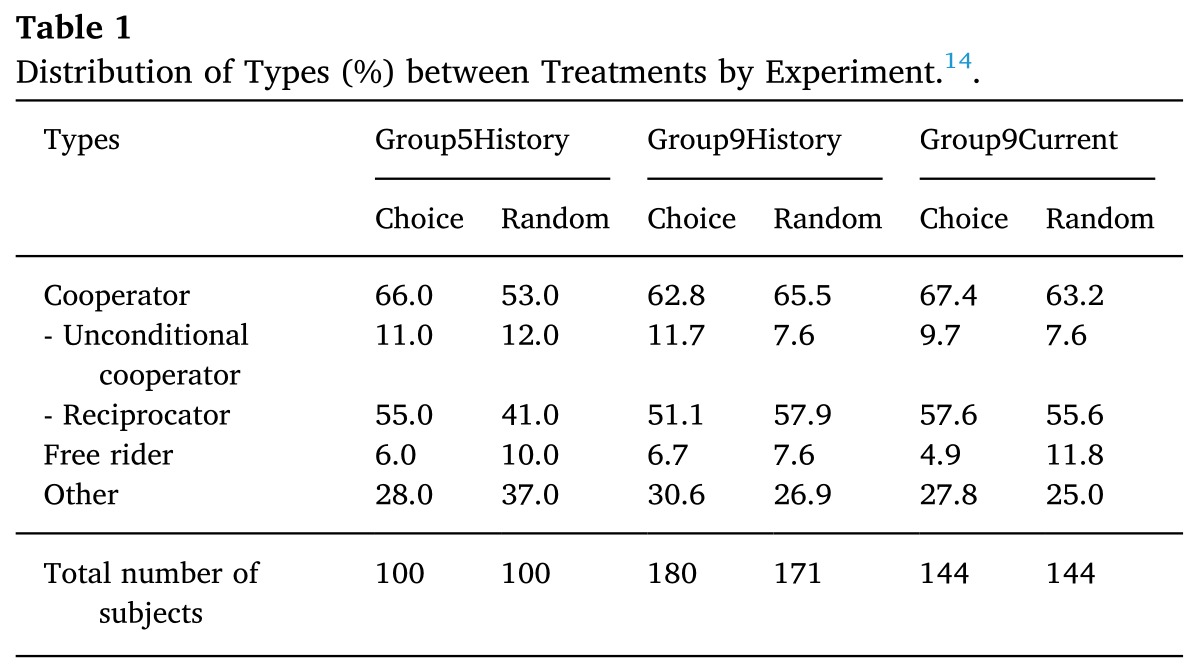
\includegraphics[width=0.9\textwidth,height=\textheight]{20220426-serdarevic-nina-it-pays-to-be-nice.assets/image-20220425210127736.png}
\caption{Distribution of Types}
\end{figure}
\end{frame}

\hypertarget{results}{%
\section{Results}\label{results}}

\begin{frame}{The Benefits of Being a Cooperator}
\protect\hypertarget{the-benefits-of-being-a-cooperator}{}
\begin{figure}
\centering
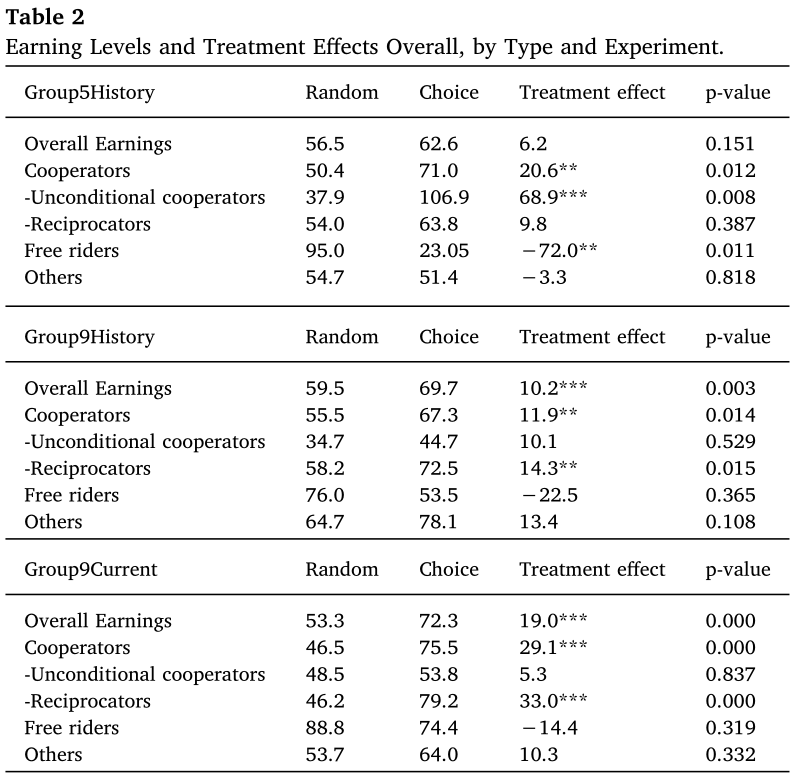
\includegraphics[width=0.8\textwidth,height=\textheight]{20220426-serdarevic-nina-it-pays-to-be-nice.assets/Pasted image 20220424001212.png}
\caption{Treatment Effects on Earning, by Type and Experiment}
\end{figure}
\end{frame}

\begin{frame}
\begin{block}{Assortativity}
\protect\hypertarget{assortativity}{}
1.2\%, 11.3\%, and 22\% higher in Choice treatment.
\end{block}

\begin{block}{Successful Mutual Matching Frequency}
\protect\hypertarget{successful-mutual-matching-frequency}{}
\begin{figure}
\centering
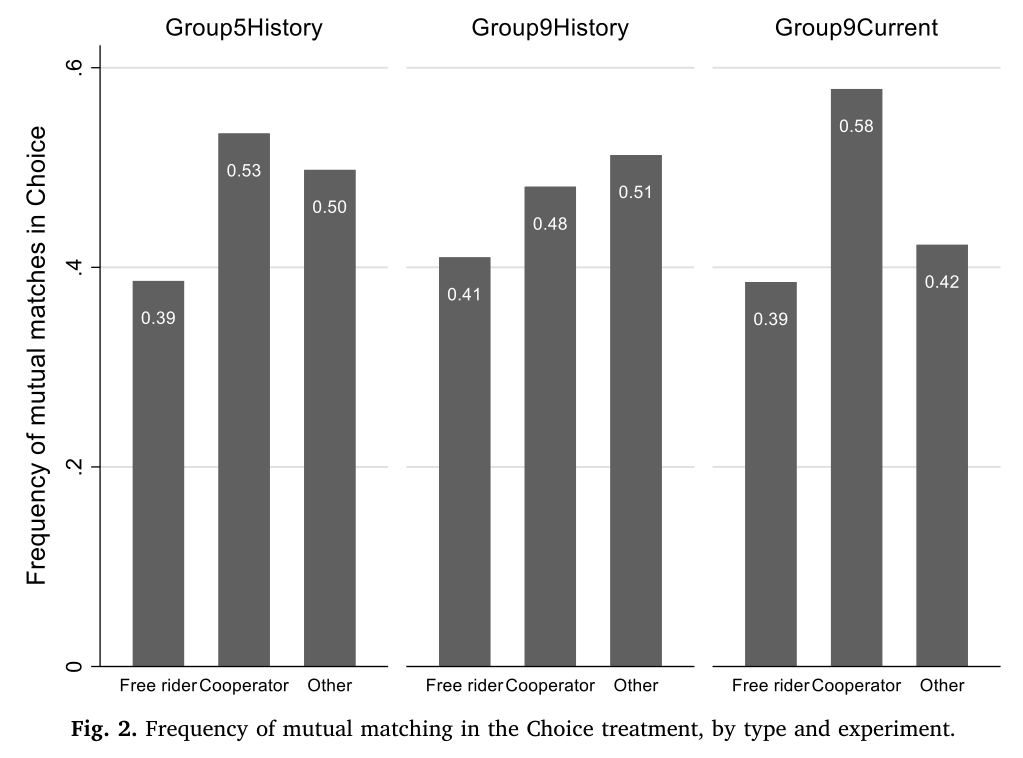
\includegraphics[width=0.7\textwidth,height=\textheight]{20220426-serdarevic-nina-it-pays-to-be-nice.assets/Pasted image 20220424001146.png}
\caption{Successful Mutual Matching Frequency}
\end{figure}
\end{block}
\end{frame}

\begin{frame}{Group Size and Reminder of Personal Reputation History}
\protect\hypertarget{group-size-and-reminder-of-personal-reputation-history}{}
\begin{figure}
\centering
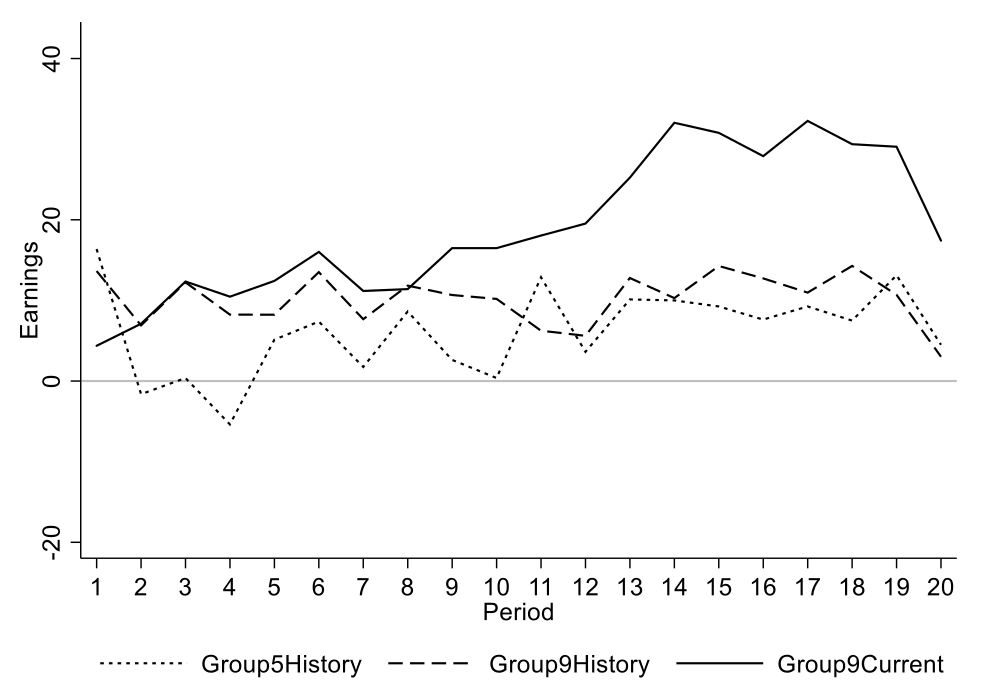
\includegraphics[width=0.6\textwidth,height=\textheight]{20220426-serdarevic-nina-it-pays-to-be-nice.assets/Pasted image 20220424001923.png}
\caption{Treatment effect on earnings, over period and by experiment
\newline \footnotesize Differences aren't significant.}
\end{figure}

\normalsize Why complete information leads to lower earning?
\emph{Search cost creates incentives for cooperation.}
\end{frame}

\hypertarget{discussion}{%
\section{Discussion}\label{discussion}}

\begin{frame}{Discussion}
\begin{block}{Choice improved cooperators' earning even with more
freeriders}
\protect\hypertarget{choice-improved-cooperators-earning-even-with-more-freeriders}{}
\begin{figure}
\centering
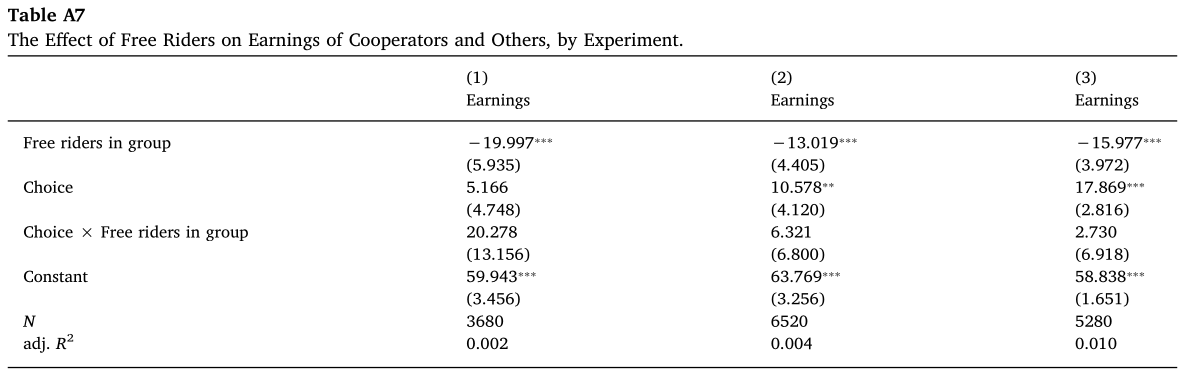
\includegraphics{20220426-serdarevic-nina-it-pays-to-be-nice.assets/Pasted image 20220424002431.png}
\caption{Effect of Free Riders on Earnings of Cooperators and Others}
\end{figure}
\end{block}
\end{frame}

\begin{frame}
\begin{block}{Free riders tends to be the one being excluded}
\protect\hypertarget{free-riders-tends-to-be-the-one-being-excluded}{}
\begin{table}
    \caption{Cooperator and its likelihood to be excluded}
    \scalebox{0.8}{
        \begin{tabular}{@{}lccc@{}}
            \toprule
                                         & \textbf{Exclusion} & \textbf{Exclusion} & \textbf{Exclusion} \\
                                         & Group5History      & Group9History      & Group9Current      \\ \midrule
            Choice                       & 0.122***           & 0.055              & 0.052*             \\
            Choice \(\times\) Cooperator & −0.144***          & −0.053             & −0.071**           \\ \bottomrule
        \end{tabular}
    }
    \caption*{Excerpted from Table A1, A3, A5}
\end{table}

\end{block}
\end{frame}

\begin{frame}
\begin{block}{Free riders do not fake itself as cooperators}
\protect\hypertarget{free-riders-do-not-fake-itself-as-cooperators}{}
\begin{table}
    \caption{Free rider and its contribution under Choice treatment}
    \scalebox{0.8}{
        \begin{tabular}{@{}lccc@{}}
            \toprule
                                         & \textbf{Contribution} & \textbf{Contribution} & \textbf{Contribution} \\
                                         & Group5History         & Group9History         & Group9Current         \\ \midrule
            Choice                       & 0.410                 & 0.875**               & 1.538***              \\
            Choice \(\times\) Free rider & −0.283                & 1.234                 & 2.151                 \\ \bottomrule
        \end{tabular}
    }
    \caption*{Excerpted from Table A1, A3, A5}
\end{table}

\end{block}
\end{frame}

\hypertarget{remarks}{%
\section{Remarks}\label{remarks}}

\begin{frame}{Remarks}
\begin{enumerate}
\tightlist
\item
  Partner choice is good for cooperators, bad for free riders.
\item
  Cooperators have higher probability of matching a cooperator, and less
  being excluded from the game.
\item
  Partner choice effect is greater at ``large'' society (although not
  significant)
\item
  Altruism might be an evolutionarily stable strategy (ESS) in
  competitive partnering market.
\end{enumerate}
\end{frame}

\end{document}
